\documentclass{exampaper}
\usepackage{graphicx, ulem, paralist, float, subfigure}

\examtitle{Minecraft红石等级测试}
\cotitle{一级 \qquad \uline{生}存用\uline{电}路}
\date{}

\begin{document}
    \maketitle

    % 注意事项
    \begin{material}
        \noindent \heiti 注意事项: \songti

        \begin{compactenum}
            \item 本卷满分100分,测试时间60分钟。
            \item 本卷中所有使用到的游戏特性均以Minecraft Java Edition 1.18.2版本为准。
            \item 本卷中所有设施运行结果均应当为其运行在$TPS=20.0$情况下的结果为准。
            \item 单位gt是gametick的缩写,1gt代表一个游戏刻。单位rt是redstonetick的缩写,代表一个红石刻,默认情况下$1rt=2gt$。
            \item 上机操作题建议在服务器中完成,无法在服务器中完成的,可以提交上机操作的全程录屏。
            \item 上机操作题应当使用创造模式进行完成。
        \end{compactenum}
    \end{material}

    \part{客观题}
        \section{选择题}{共10题,每题5分}
            \subsection{生电是\dash{1cm}的简称。}
                \fourselections{生存用电路}{生产线电路}{生活电路}{妈妈生的电路}
            
            \subsection{以下哪一类红石设施不属于生电的范畴。}
                \fourselections{红石计算机}{全自动刷怪塔}{刷地毯机}{烤鸡机}
            
            \subsection{以下哪个方块是不可充能方块?}
                \fourselections{石头}{玻璃}{混凝土}{木板}
            
            \subsection{如图,要使得红石火把\dotuline{熄灭},应当在\textbf{蓝色羊毛}处放置什么方块?}
                \fourselections{石头或圆石}{羊毛或树叶}{玻璃或混凝土}{红石比较器}
            
            \subsection{小明刚刚学习红石,他尝试自己制作了一个高频红石发生器,但不知道为什么没有产生高频红石信号,请你帮他\dotuline{找出问题所在}。}
                \twoselections{比较器未设置为比较模式}{红石线路没铺对}{比较器未设置为减法模式}{游戏Bug}
            
            \subsection{要使得图中的铁轨正常转向,应当将\textbf{蓝色羊毛上的方块}替换为什么方块?}
                \fourselections{动力铁轨}{探测铁轨}{铁轨}{激活铁轨}
            
            \subsection{Steve和Alex是好伙伴,他们两于 \today 进行了赛船比赛。比赛前,Alex把她的赛道上的水换成了蓝冰,请问谁会先到达终点?}
                \fourselections{Steve}{Alex}{同时到达}{随缘}
            
            \clearpage

            \subsection{红石中继器的延迟最大可以设置为\dash{1cm},最小可以设置为\dash{1cm}。}
                \fourselections{$2rt$;$1rt$}{$4rt$;$2rt$}{$4gt$;$1gt$}{$4rt$;$1rt$}
            
            \subsection{阅读材料,解释为何本卷\textbf{注意事项}中设定所有设施运行结果均应当为其运行在$TPS=20.0$情况下的结果为准。}
                \vspace{0.25cm}
                \begin{material}
                    Minecraft的绝大多数计算逻辑都在一个游戏循环内执行,执行一次这个循环就被称为执行了一次游戏刻(Game Tick),作为单位时缩写为gt。

                    由于游戏不能时刻都在计算而消耗资源,所以游戏刻执行一次后线程会进行休眠,等待下一次执行,从而维持一秒内游戏刻的执行次数相等且均匀。通常情况下,每秒最多运行20次游戏刻,即从这一游戏刻开始执行到下一游戏刻执行的时间间隔为0.05秒。如果这次游戏刻计算时间小于两个游戏刻的时间间隔,则会进行休眠直到下一游戏刻的执行。
                    
                    —— Minecraft Wiki
                \end{material}
                \vspace{0.25cm}

                \twoselections{MRLT编写组乱写的}{TPS过低会影响机器运行结果}{$TPS\neq 20$时游戏会崩溃}{TPS是一个常量,始终等于20}
            
            \subsection{当我们希望查询有关Minecraft的知识时,应当前往哪个网站?}
                \vspace{0.25cm}
                \begin{material}
                    致各位读者:

                    大家好!我们很高兴宣布,中文Minecraft Wiki已经从Fandom迁移到zh.minecraft.wiki了——一切与Minecraft有关的信息,在新地方应有尽有!

                    —— Minecraft Wiki
                \end{material}
                \vspace{0.25cm}

                \twoselections{https://zh.minecraft.wiki/}{https://minecraft.fandom.com/}{https://minecraft.net/}{https://mc.163.com/}
            
            % 图片区
            \begin{figure}[H]
                \centering
                \vspace{-0.35cm}
                \subfigtopskip=2pt
                \subfigbottomskip=2pt
                \subfigcapskip=-5pt

                \subfigure[第4题图]{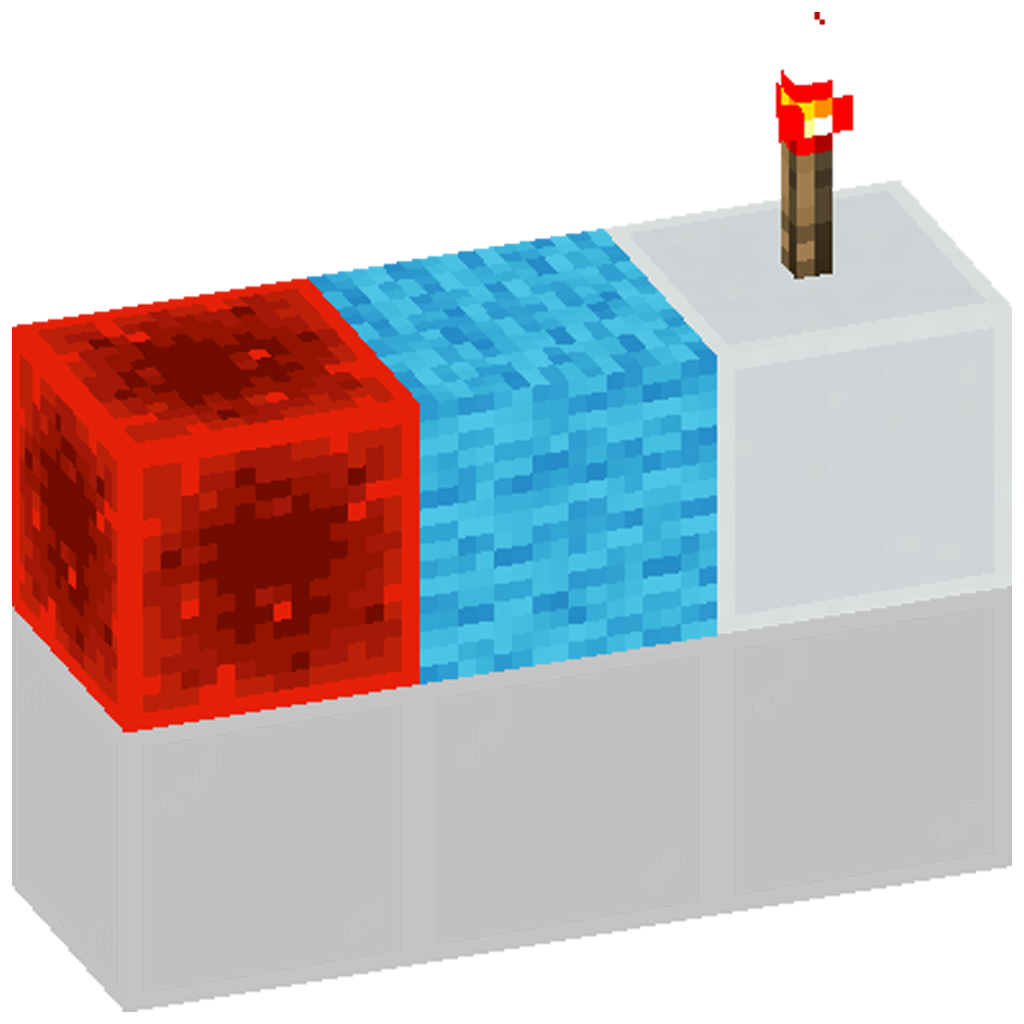
\includegraphics[width=2cm]{images/L1/Q4.png}}
                \quad
                \subfigure[第5题图]{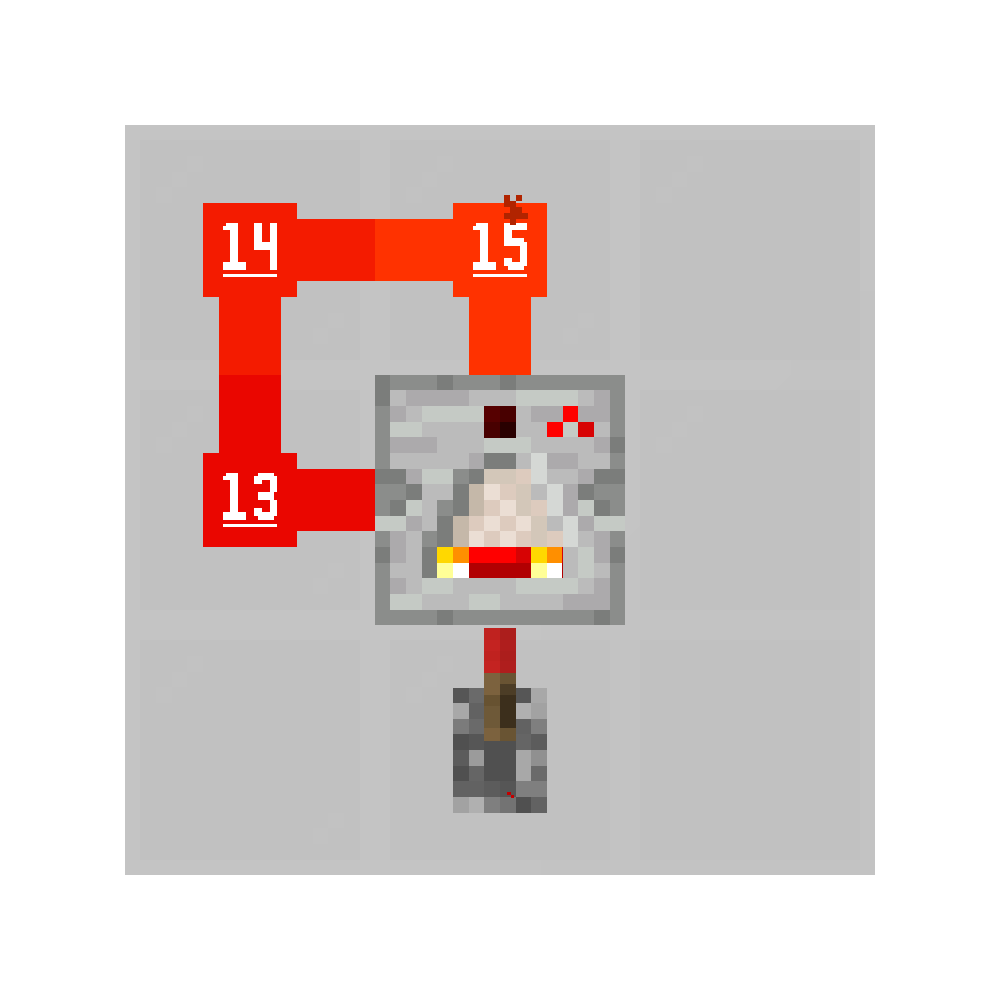
\includegraphics[width=2cm]{images/L1/Q5.png}}
                \quad
                \subfigure[第6题图]{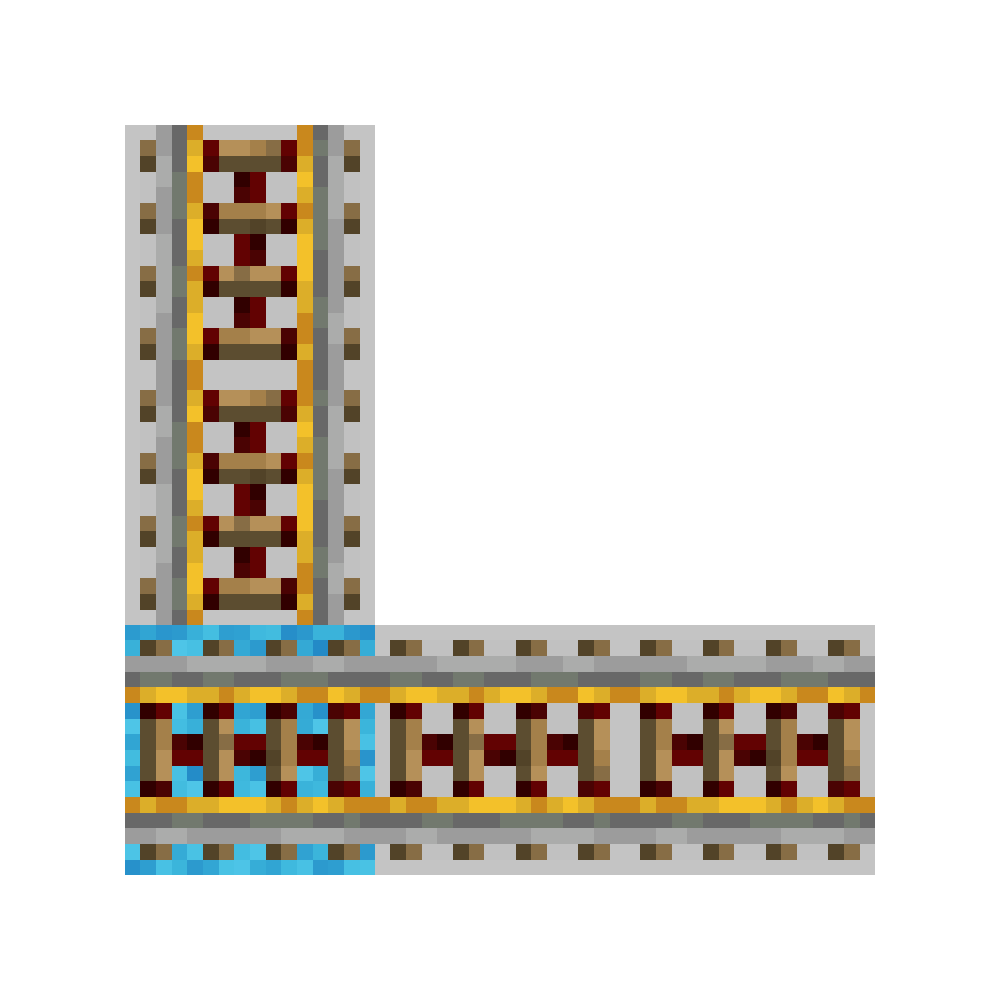
\includegraphics[width=2cm]{images/L1/Q6.png}}
                \quad
                \subfigure[第7题图]{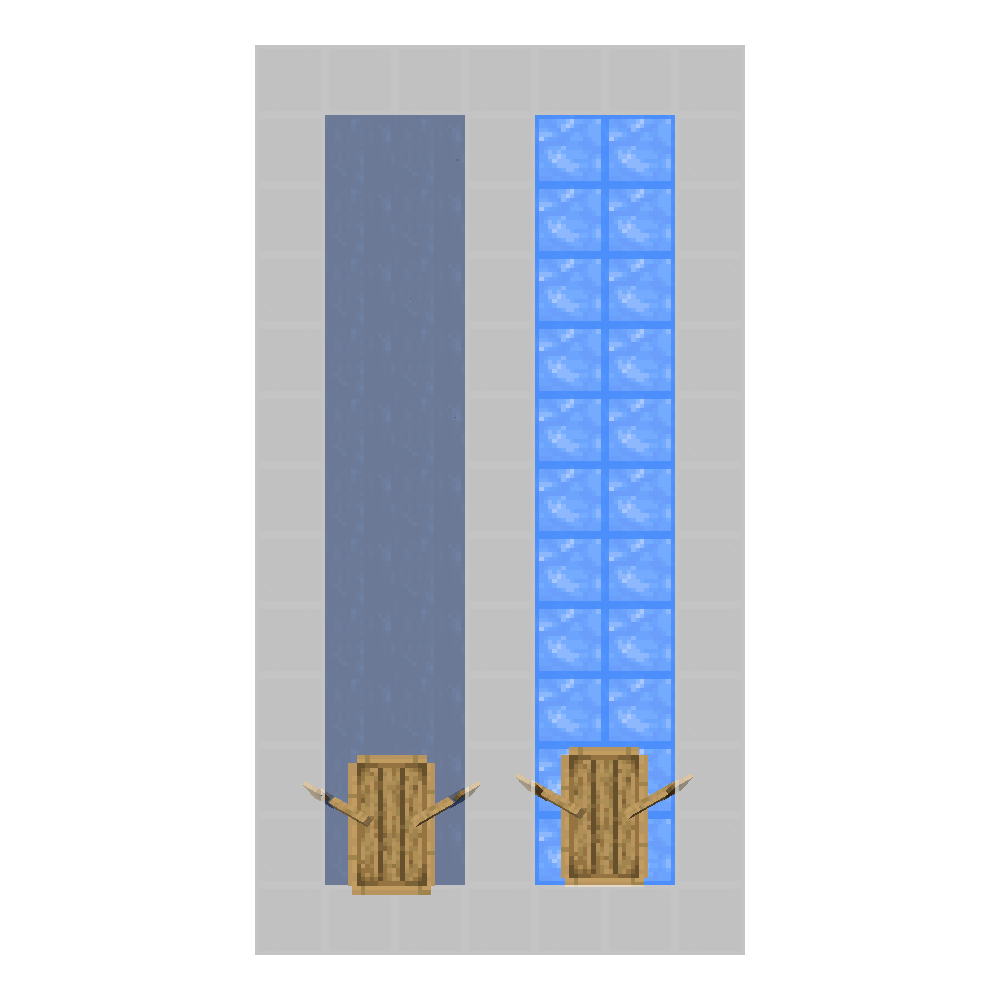
\includegraphics[width=2cm]{images/L1/Q7.png}}
            \end{figure}

        \clearpage

    \part{主观题}
        \section{阅读材料,回答问题}{共2题,每题10分}
            \begin{material}
                在Minecraft的非和平难度下,每一位玩家都有相应的“刷怪上限”(详见生成)。当且仅当相应维度中所有被加载的区块内未被命名、未乘坐矿车或船、未拾起过掉落物的敌对生物总数小于总的刷怪上限时,大部分敌对生物才会自然生成。正常而言,相应维度内距离玩家128格以外的敌对生物会立即消失,但处于非强加载区块内的则是例外。其中,处于弱加载区块内的敌对生物会记入世界中敌对生物总数。因此,在特定区域内囤积足够的敌对生物,配合基于下界传送门的区块加载器,便可在主世界和下界禁止大部分敌对生物自然生成。—— Minecraft Wiki
            \end{material}

            \subsection{小明希望在一个大型生电服务器中实现伪和平,但在未与其他玩家沟通的情况下擅自搭建了伪和平装置,结果他的伪和平装置遭到了拆除。请你结合材料简单分析,为什么小明的的伪和平装置会被拆除?}
                \vspace{2cm}
            
            \subsection{搭建伪和平装置会导致服务器中的哪些生电设施无法使用?}
                \vspace{2cm}
        
    \part{上机操作题}
        \section{运用所学知识,设计红石装置}{共5个评分点,每个评分点6分}
            题目背景:Alex觉得Minecraft中的熔炉加工矿石速度太慢,请你帮Alex设计一个高速熔炉。

            帮助信息:熔炉上方的漏斗可以向熔炉输入待加工物,后方的漏斗可以向其输入燃料,下方的漏斗可以输出产物。同时,漏斗也可以从上方箱子矿车中吸取物品。

            评分点如下:

            \subsection{可以一次性放入5组待加工物品。}

            \subsection{可以一次性放入27组待加工物品。}

            \subsection{输出物品可以集中到一个容器内。}

            \subsection{熔炉倍速>=10x。}

            \subsection{【高难度】输出物品可以自动打包到潜影盒内。}
\end{document}